\chapter{Mobile Application Development}
\label{chp:mobile_app}

\par The source code of \gls{ios} application is on the Github public repository \url{https://github.com/br1anchen/WifiAccessManager_IOS}. The \gls{ios} project is developed under \gls{macos} 10.8.5 by Xcode 5.0.1 using \gls{ios} 7 \gls{sdk}. The programming language using in this application is Objective-C\cite{objc}, it is a general-purpose, object-oriented programming language that adds Smalltalk-style messaging to the C programming language. It is the main programming language used by Apple for the OS X and iOS operating systems and their respective APIs, Cocoa and Cocoa Touch.The improved Android application's source code is also on the Github public repository \url{https://github.com/br1anchen/WifiAccessManager_Android}. It is developed under \gls{macos} 10.8.5 by \gls{adt}.

\section{IOS Wifi Access Manager Application}

\par During the development period of \gls{ios} management application, Apple just released new \gls{ios} \gls{sdk},which is \gls{ios} 7 on all the \gls{ios} devices. And the new Xcode \gls{ide} is upgraded with this new \gls{sdk} library as well. So for this prototype project, \gls{ios} application is developed under these \gls{sdk} scope. Because of the time limit for this project and the main goal of it is not to provide advanced mobile application, some necessary feature like user interface design will not be considered as high priority in this project. Furthermore, it is simple management application for prototype, it will not include highly advanced software design architecture.

\subsection{SDK Library Using in IOS Wifi Access Manager Application}
\par There are three key \gls{sdk} library using in this project. 

\subsubsection{Foundation.framework}
\par The first one is Foundation Framework library \cite{foundationlib},it defines a base layer of Objective-C classes. In addition to providing a set of useful primitive object classes, it introduces several paradigms that define functionality not covered by the Objective-C language. It is designed with these goals in mind:
\begin{itemize}
  \item Provide a small set of basic utility classes.
  \item Make software development easier by introducing consistent conventions for things such as deallocation.
  \item Support Unicode strings, object persistence, and object distribution.
  \item Provide a level of OS independence, to enhance portability.
\end{itemize}
\par Most of the \gls{ios} application is based on this important library because it includes the root object class, classes representing basic data types such as strings and byte arrays, collection classes for storing other objects, classes representing system information such as dates, and classes representing communication ports.

\subsubsection{CoreGraphics.framework}
\par The second library is Core Graphics Framework library \cite{coregraphicslib}. It is a C-based API that is based on the Quartz advanced drawing engine. It provides low-level, lightweight 2D rendering with unmatched output fidelity. You use this framework to handle path-based drawing, transformations, color management, offscreen rendering, patterns, gradients and shadings, image data management, image creation, masking, and PDF document creation, display, and parsing. In this project, the application's request list swiping to approve or block gesture animation is based on this library although this customized user interface component is also based on the other third party class library. The working animation result is shown in Figure \ref{fig:ios_swipe}.

\subsubsection{UIKit.framework}
\par The third \gls{sdk} library using in the project is UIKit Framework library \cite{uikitlib}. It provides the classes needed to construct and manage an application’s user interface for iOS. It provides an application object, event handling, drawing model, windows, views, and controls specifically designed for a touch screen interface. Since mobile applications require very high responsiveness for user interface event, this library will provide all these kind of event to the application logic system to handle with. For example, the swipe gesture in this application, it will dispatch an user interface swipe event to the run-time system, and the touch event on the login button will dispatch another event to the run-time system as well.

\subsection{Third Party Library Using in IOS Wifi Access Manager Application}

\par Although the native \gls{sdk} \gls{ios} 7 library provided by Apple is quite powerful and convenient to use, there are still some process missing or not good enough to work with. Then third party library provided as open source project is necessary to use in this application.

\subsubsection{UITableViewCell-Swipe-for-Options}
\par In order to make the managing process of the client requests approving or blocking more convenient to use, the similar gesture function using in \gls{ios} 7 Mail App is a good solution for administrator to approve or block a client request in the connect device list by just swiping the corresponding list row and choose the approve or block button to make the management command to server. This open source project,UITableViewCell-Swipe-for-Options\cite{swipe-for-options}, hosted on Github is better choice in this project to replace with the normal UITableViewCell component( which is default table row component in \gls{ios} user interface).

\subsubsection{JSONKit}
\par JSONKit\cite{jsonkit} is a very high performance Objective-c \gls{json} Library. Although in \gls{ios} 7 \gls{sdk}, it provides the simple \gls{json} parsing and serializing function. But it is limited with complexity of the \gls{json} object needed to be parsed or serialized. In this project, the \gls{json} object using during the communication between mobile client and server is quite complicated data structure object, so by using this third party \gls{json} library is easier for developer to program the application. Moreover, the performance of the JSONKit to parse data to \gls{json} object or serialize the \gls{json} object to Objective-c object is better than any \gls{json} framework in \gls{ios} application development scope.

\subsubsection{Base64}
\par Base64\cite{base64lib} is a set of categories that provide methods to encode and decode data as a base-64-encoded string. Because of the security login mechanism is implemented on the central management server, it is required for \gls{ios} mobile application to have Base64 encoding process. The third party Base64 library is introduced for this reason.

\subsection{Structure of IOS Wifi Access Manager Application}

\subsubsection{Story Board}

\begin{figure}
	\centering
    	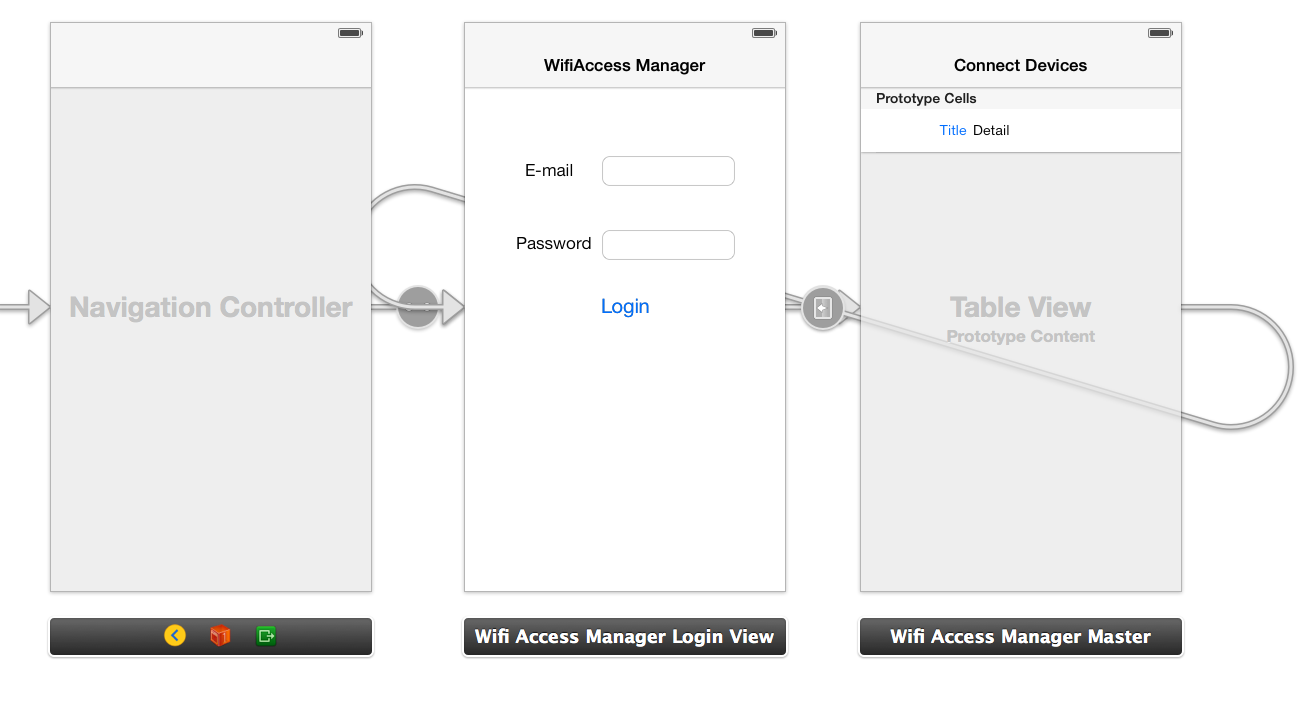
\includegraphics[width=0.80\textwidth,natwidth=610,natheight=642]{figs/ios_app_storyboard.png}
  	\caption{IOS Mobile Application Story Board Design}
  	\label{fig:ios_storyboard}
\end{figure}

\par Storyboard\cite{xcode_storyboard} is a visual representation of the user interface of an iOS application, showing screens of content and the connections between those screens. A storyboard is composed of a sequence of scenes, each of which represents a view controller and its views; scenes are connected by segue objects, which represent a transition between two view controllers.

\par Xcode provides a visual editor for storyboards, where you can lay out and design the user interface of your application by adding views such as buttons, table views, and text views onto scenes. In addition, a storyboard enables you to connect a view to its controller object, and to manage the transfer of data between view controllers. Using storyboards is the recommended way to design the user interface of your application because they enable you to visualize the appearance and flow of your user interface on one canvas.

\par The story board design of the \gls{ios} application is shown in Figure \ref{fig:ios_storyboard}. There are only two visible view in the story board, which are Wifi Access Manager Login View and Wifi Access Manager Master View. The view controller to push or pop user interface view to the font scene is navigation controller. Wifi Access Manager Login View is the place for administrator of the internet access control system to login the mobile application. And the Wifi Access Manager Master view is a subview of the UITableView(the user interface view class in \gls{ios}), it consists a list of the connected devices in the residential wireless network with status of each device's access request.

\subsubsection{View Controllers}
\par Since there are two views in the application, each of them has their own view controller to handle the user interface event with the corresponding application logic function. 
\par The view controller for Login View shown in Figure \ref{fig:ios_login_page} and Figure \ref{fig:ios_login_process} is WifiAccessManagerLoginViewController. The userLogin function (the main application logic function in WifiAccessManagerLoginView) is display in the Code Snippet \ref{code:ios_userlogin}. In this function, it takes the values from the user interface input as E-mail and password, then use the helper class which will be discussed later in this chapter to make the \gls{http} post request to the central management server to check the user authentication. If the login is successful it will use the story board 'performSegueWithIdentifier' function to get the corresponding segue by the name 'afterLogin'. The login process is shown in Figure \ref{fig:ios_login_process} After that this segue will be triggered, which is to push the Wifi Access Manager Master view to the font scene. Also the administrator login information will be stored as user profile in this application sandbox folder, it can be used for later multitask switching application process on \gls{ios} from other application to make the application no need to login again.

\begin{algorithm}[h]
\floatname{algorithm}{Code Snippet}
  \caption{userLogin function in WifiAccessManagerLoginViewController.m}
  \label{code:ios_userlogin}
  \begin{verbatim}
  
- (IBAction)userLogin:(id)sender {
    self.email = self.email_input.text;
    self.password = self.pwd_input.text;
    
    NSString *loginInfo = 
    		[NSString stringWithFormat:
    			@"WifiAccess Manager:Login:email: %@, pwd: %@",
    			self.email,self.password];
    NSLog(@"%@", loginInfo);
    
    HttpRequestUtilities *httpHelper = [[HttpRequestUtilities alloc] init];
    
    if([httpHelper loginRequest:self.email withPassword:self.password])
    {
        NSLog(@"Login Success.");
        NSUserDefaults *userPref = [NSUserDefaults standardUserDefaults];
        [userPref setValue:self.email forKey:@"Email"];
        [userPref synchronize];
        
        [self performSegueWithIdentifier: @"afterLogin" sender: self];
    }else{
        NSLog(@"Login Failed.");
        UIAlertView *loginAlert = 
        		[[UIAlertView alloc] 
        			initWithTitle:@"Login Failed" 
        			message:@"Please check your user information then login again" 
        			delegate:self 
        			cancelButtonTitle:@"OK" 
        			otherButtonTitles:nil,nil];
        [loginAlert show];
    }
}

 \end{verbatim}
\end{algorithm}

\begin{figure}
	\centering
	\begin{minipage}{0.45\textwidth}
		\centering
    		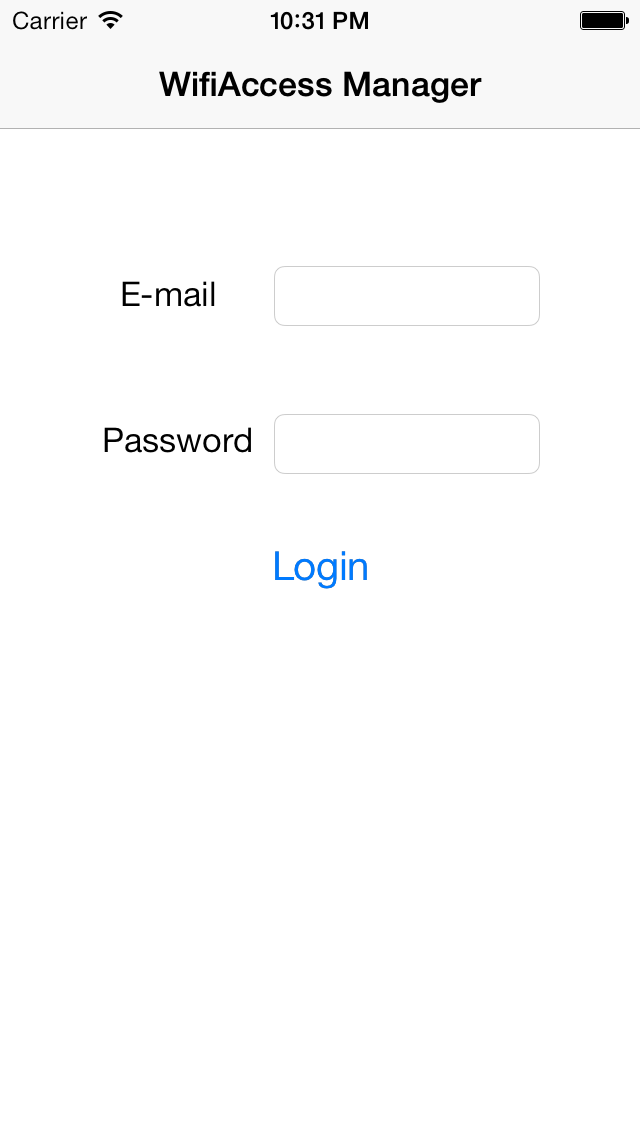
\includegraphics[width=0.6\textwidth,natwidth=610,natheight=642]{figs/ios_app_login_page.png}
  		\caption{IOS Mobile Application Login View}
  		\label{fig:ios_login_page}
  	\end{minipage}
  	\hfill
  	\begin{minipage}{0.45\textwidth}
  		\centering
  		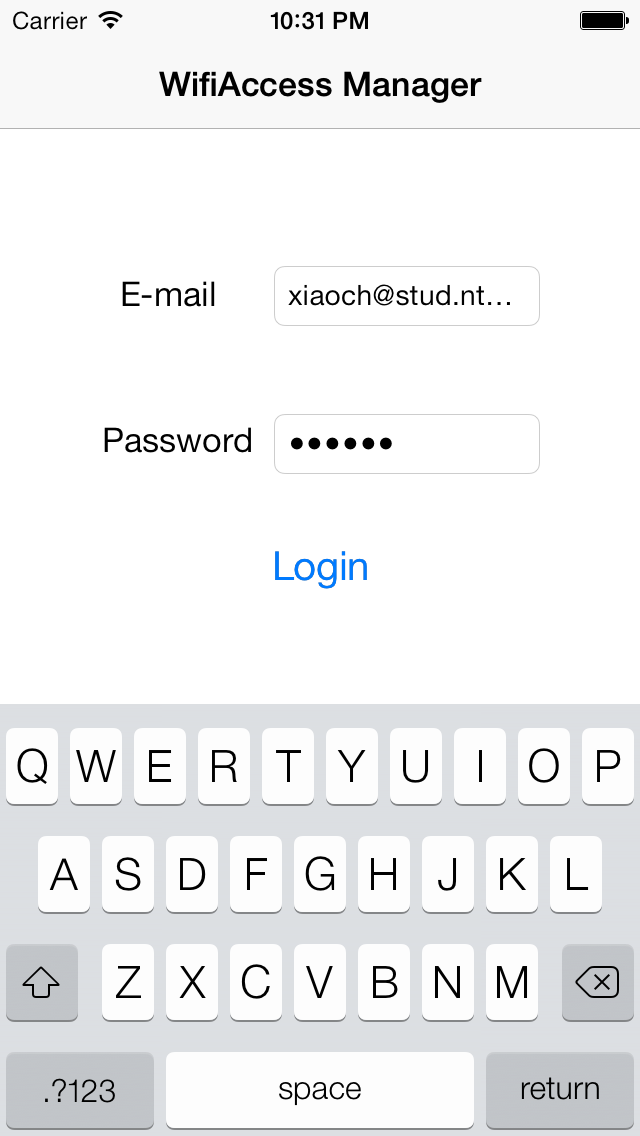
\includegraphics[width=0.6\textwidth,natwidth=610,natheight=642]{figs/ios_app_login_process.png}
  		\caption{IOS Mobile Application Login Process}
  		\label{fig:ios_login_process}
  	\end{minipage}
\end{figure}

\begin{figure}
	\centering
	\begin{minipage}{0.45\textwidth}
  		\centering
  		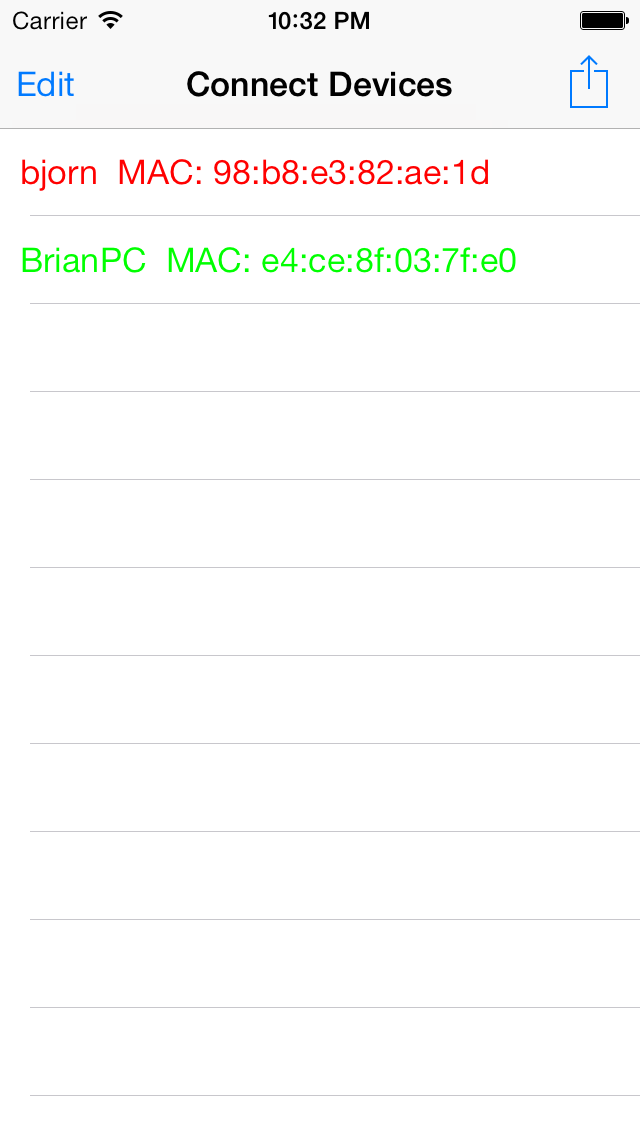
\includegraphics[width=0.6\textwidth,natwidth=610,natheight=642]{figs/ios_app_request_list.png}
  		\caption{IOS Mobile Application Request List View}
  		\label{fig:ios_requests}
  	\end{minipage}
  	\hfill
	\begin{minipage}{0.45\textwidth}
		\centering
    		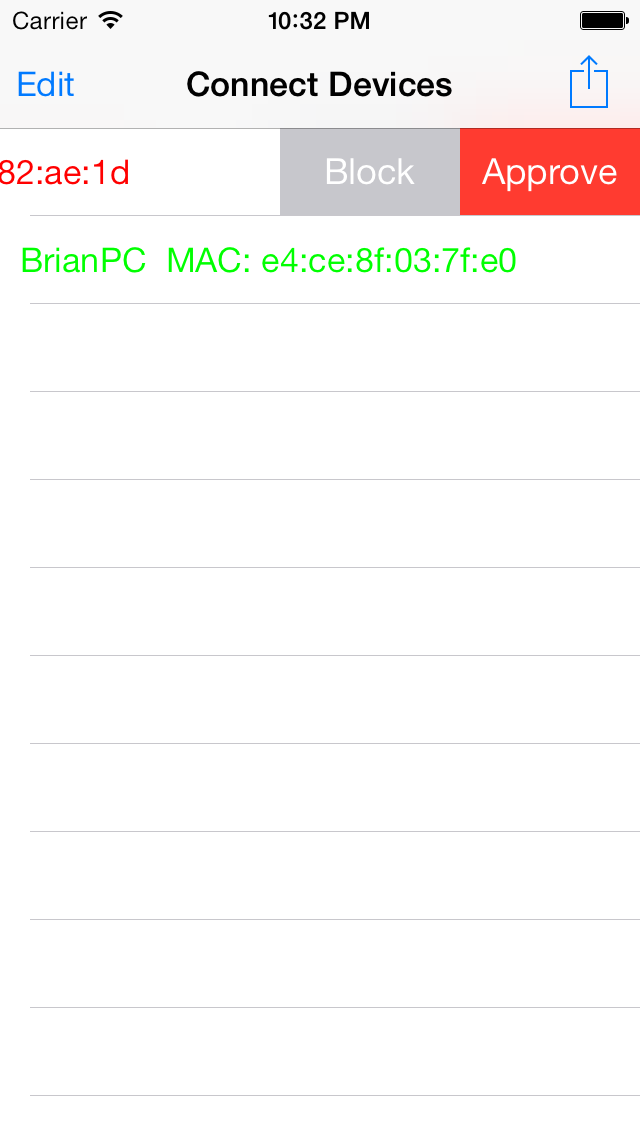
\includegraphics[width=0.6\textwidth,natwidth=610,natheight=642]{figs/ios_app_manage_gesture.png}
  		\caption{IOS Mobile Application Swipe Gesture}
  		\label{fig:ios_swipe}
  	\end{minipage}
\end{figure}

\par The view controller for Wifi Access Manager Master view is more complicated than Wifi Access Manager Login View because it includes a UITableView, swipe gesture function with approve and block request function and automatic updating function in it. Because this view is a table view then this view controller is a sub-view controller  class of UITableViewController. It will have the delegate functions from the UITableViewController to controll the table view. Moreover it will have the delegate functions from third party library,TLSwipeForOptionsCellDelegate, to make the swipe to options function working on cell components in the table view. The loadTableData function in Code Snippet \ref{code:ios_loadtabledata} of Appendix \ref{chp:appendix2}, is the function to get the request lists from the server. It call the helper class 'HttpRequestUtilities' to make the \gls{http} post request to the central management server to get all the requests for the corresponding administrator. Then using the \gls{json} serialization to convert the \gls{json} object array to the objective-c NSMutableArray for displaying in the table view. But since the mechanism of \gls{ios} is to not block the user interface thread all the time, so this load table data will be run as another separate thread, after fetching the data from the server, reloadData function of self.tableView needs to be called to force the table content refresh with the new fetching data. The result after this process is shown in Figure \ref{fig:ios_requests}.

\par The automatic updating function is implemented as a timer repeat in 10 second interval to call the loadTableData function in the application. The implementation code is shown in Code Snippet \ref{code:ios_updatetimer}.

\begin{algorithm}[h]
\floatname{algorithm}{Code Snippet}
  \caption{timer code in WifiAccessManagerMasterViewController.m}
  \label{code:ios_updatetimer}
  \begin{verbatim}
  
    updateTimer = [NSTimer scheduledTimerWithTimeInterval:10 
    							target:self 
    							selector:@selector(loadTableData) 
    							userInfo:nil 
    							repeats:YES];
    [updateTimer fire];
 \end{verbatim}
\end{algorithm}

\begin{figure}
	\centering
	\begin{minipage}{0.45\textwidth}
		\centering
    		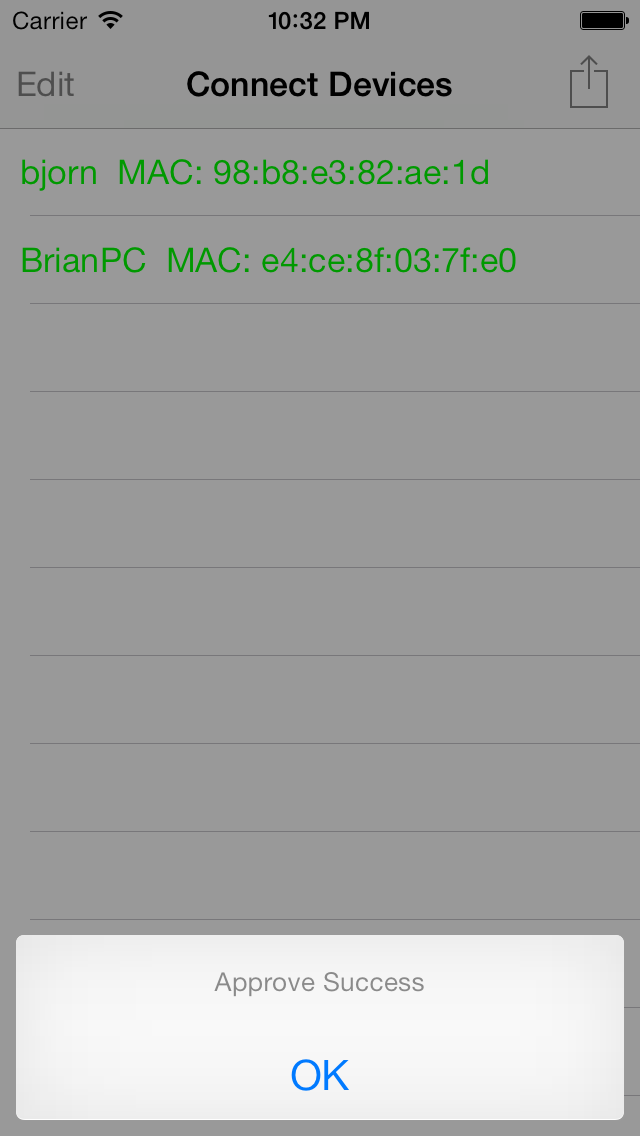
\includegraphics[width=0.45\textwidth,natwidth=610,natheight=642]{figs/ios_app_approve_request.png}
  		\caption{IOS Mobile Application Approve Request Process}
  		\label{fig:ios_approve}
  	\end{minipage}
  	\hfill
  	\begin{minipage}{0.45\textwidth}
  		\centering
		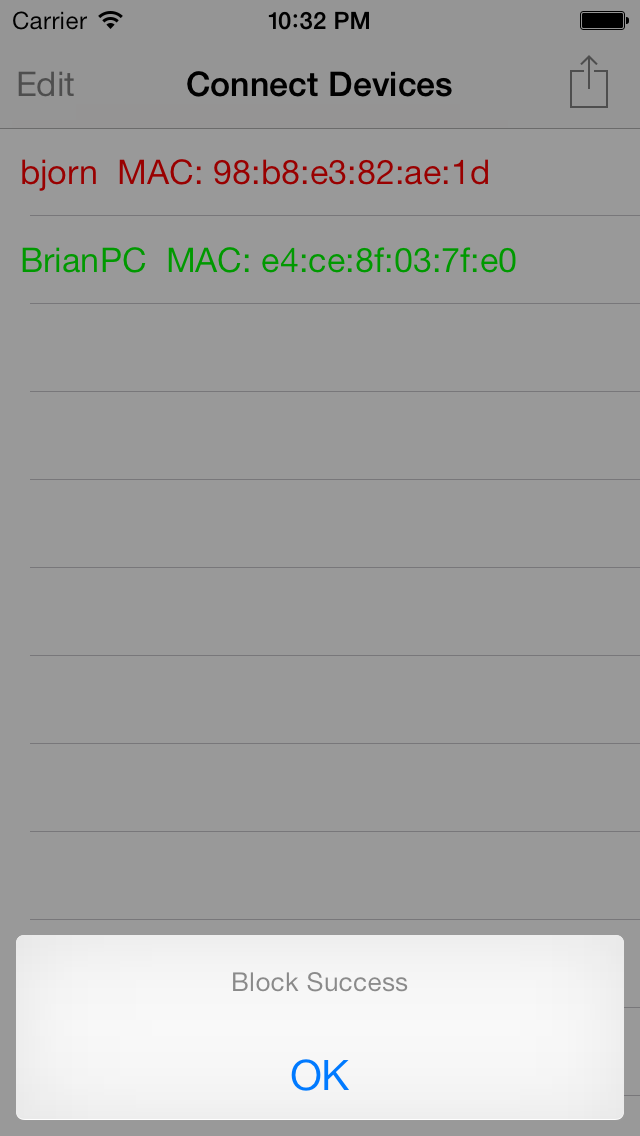
\includegraphics[width=0.45\textwidth,natwidth=610,natheight=642]{figs/ios_app_block_request.png}
  		\caption{IOS Mobile Application Block Device Process}
  		\label{fig:ios_block}
  	\end{minipage}
\end{figure}

\par The approving and blocking process shown in Figure \ref{fig:ios_approve} and Figure \ref{fig:ios_block} is implemented by the similar function in the WifiAccessManagerMasterViewController. In this report, only approve function displayed in Code Snippet \ref{code:ios_approve} of Appendix \ref{chp:appendix2} will be discussed as code sample of these application process. This function is a delegate function from TLSwipeForOptionsCell class, which provide the method to get current select row of the table view to do further application process. The 'cellDidSelectApprove' function in this application will get the corresponding data from the current selected row to make the \gls{http} post request to post the changes for the client request status(in this case it is approving the request). Like loadTableData function mentioned before, it is thread safe process as well, so it is necessary to call the loadTableData to fetch latest data from central management server and force the table view to refresh the content.

\subsubsection{HttpRequestUtilities}
\par To make the work of development for this application easier, one helper class named as HttpRequestUtilities is made in the project. This class will use other two third party library(JSONKit,Base64) to handle all the \gls{http} request to the server. There are three different \gls{http} request in the application. They are shown as Code Snippet \ref{code:ios_http_login}, Code Snippet \ref{code:ios_http_getrequests} and Code Snippet \ref{code:ios_http_postclient} in the Appendix \ref{chp:appendix2}. They are main \gls{http} communication between the mobile application client and central management server.All of them are quite similar, the function set an \gls{url} with the corresponding address string, then create a  NSMutableURLRequest object to set all the corresponding information data in \gls{http} request header or body, then make the NSURLConnection with the central server to get the response back.

\section{Improvement for Android Application}
\par Because of the security login mechanism on the central management server, there will be some changes on Android Application as well. By using the android.util.Base64 library, the encoding user name and password process is implemented. In the previous master project, there is no login parameter for password, so it needs to add for Android Application. The main changes is shown in the Code Snippet \ref{code:android_login}.

\begin{algorithm}[h]
\floatname{algorithm}{Code Snippet}
  \caption{login changes on Android Application}
  \label{code:android_login}
  \begin{verbatim}
  
Map<String, String> loginParams = new HashMap<String, String>();
loginParams.put("email", 
		Base64.encodeToString(mEmail.getBytes(), Base64.DEFAULT));
loginParams.put("password", 
		Base64.encodeToString(mPassword.getBytes(), Base64.DEFAULT));
 \end{verbatim}
\end{algorithm} 